\documentclass[german,11pt]{beamer}
% ------------------------------------------------------------------------------
% Packages
\usepackage[german,english,french]{babel}
\usepackage[T1]{fontenc}
\usepackage[utf8]{inputenc}
\usepackage{ragged2e}
\usepackage[normalem]{ulem}


\usepackage{listings}
\usepackage{color}
\usepackage{xcolor} 
\usepackage{plantuml}
% \usepackage{enumitem} \setitemize{leftmargin=*}   // Keine Aufzählung
\usepackage{pgfplots}

\usepackage{csquotes}

\pgfplotsset{compat=1.18}

\definecolor{dkgreen} {rgb}{0,0.6,0}
\definecolor{gray}{rgb}{0.5,0.5,0.5}
\definecolor{mauve}{rgb}{0.58,0,0.82}

\lstset{frame=tb,
  language=Java,
  aboveskip=3mm,
  belowskip=3mm,
  showstringspaces=false,
  columns=flexible,
  basicstyle={\small\ttfamily},
  numbers=none,
  numberstyle=\tiny\color{gray},
  keywordstyle=\color{blue},
  commentstyle=\color{dkgreen},
  stringstyle=\color{mauve},
  breaklines=true,
  breakatwhitespace=true,
  tabsize=3
}
% ------------------------------------------------------------------------------
% Parameters
\mode<presentation>{\usetheme{Luebeck}}
\setbeamertemplate{itemize items}[triangle]
\setbeamercovered{transparent}
\usecolortheme{dove}
\usefonttheme{serif}
\addtobeamertemplate{block begin}{}{\justifying}
% ToC
\AtBeginSection[] {
  \begin{frame}{Inhalt}
    \tableofcontents[currentsection]
  \end{frame}
}
% Headline
\makeatletter
\setbeamertemplate{headline}{%
  \leavevmode%
  \@tempdimb=2.4375ex%
  \ifnum\beamer@subsectionmax<\beamer@sectionmax%
    \multiply\@tempdimb by\beamer@sectionmax%
  \else%
    \multiply\@tempdimb by\beamer@subsectionmax%
  \fi%
  \ifdim\@tempdimb>0pt%
    \advance\@tempdimb by 1.825ex%
    \begin{beamercolorbox}[wd=.5\paperwidth,ht=\@tempdimb]{section in head/foot}%
      \vbox to\@tempdimb{\hfill\insertsectionnavigation{.3\paperwidth}\vfil}%
    \end{beamercolorbox}%
    \begin{beamercolorbox}[wd=.3\paperwidth,ht=\@tempdimb]{subsection in head/foot}%
      \vbox to\@tempdimb{\vfil\insertsubsectionnavigation{.5\paperwidth}\vfil}%
    \end{beamercolorbox}%
    \begin{beamercolorbox}[wd=.2\paperwidth,ht=\@tempdimb]{subsection in head/foot}%
      \vbox to\@tempdimb{\vfil\hfill
\includegraphics[height=1cm]{fig/graphics/logo.jpg}\vfil}
    \end{beamercolorbox}%    
  \fi%
}
\makeatother
% Footline
\makeatletter
\setbeamertemplate{footline}{%
  \leavevmode%
  \hbox{\begin{beamercolorbox}[wd=.5\paperwidth,ht=2.5ex,dp=1.125ex,leftskip=.3cm,rightskip=.3cm]{author in head/foot}%
    \usebeamerfont{author in head/foot}\insertshortdate \hfill \insertshortauthor
  \end{beamercolorbox}%
  \begin{beamercolorbox}[wd=.5\paperwidth,ht=2.5ex,dp=1.125ex,leftskip=.3cm,rightskip=.3cm plus1fil]{title in head/foot}%
    \usebeamerfont{title in head/foot}\insertshorttitle \hfill \insertframenumber\,/\,\inserttotalframenumber
  \end{beamercolorbox}}%
  \vskip0pt%
}
\makeatother

\addto\captionsenglish{% Replace "english" with the language you use
  \renewcommand{\contentsname}%
    {Whatever}%
}

% ------------------------------------------------------------------------------
% Infos
\title[VS]{Verteilte Systeme}
%\subtitle[Short subtitle]{Subtitle}
\author[BCK]{Prof. Dr. Martin Becke}
\date[0.9]{Version 0.9}
\institute[CaDS]{CaDS - HAW Hamburg}
%\logo{
\includegraphics[height=1cm]{fig/graphics/logo.jpg}}
% ------------------------------------------------------------------------------

% Document
\begin{document}

% ------------------------------------------------------------------------------
% Titlepage
\begin{frame}
  \titlepage{}
\end{frame}
% ------------------------------------------------------------------------------
% ToC
%\begin{frame}{Contents}
%  \tableofcontents
%\end{frame}
% ------------------------------------------------------------------------------
\section{Supporting Patterns II} 
%\section{Einleitung}
\subsection{Dependency Injection}
\begin{frame}
  \frametitle{Dependency Injection}
  \framesubtitle{Idee}
  \begin{itemize}
    \item Abhängigkeiten eines Objekts wird von außen bereitgestellt
    \item Code wird modularer, testbarer und wartbarer
    \item Gleichen Vorteile wie das Factory Pattern
    \item Führt zusätzliche Komplexität ein 
    \item Leistung kann reduziert werden, wenn Abhängigkeiten über das Netzwerk transportiert werden muss
    \item Kann Sicherheitsprobleme einführen
    \item Problematisch im Debugging
  \end{itemize}
\end{frame}

\begin{frame}[fragile]
  \frametitle{Dependency Injection}
  \framesubtitle{Umsetzung in Code I}
  \begin{minipage}{\textwidth}
  \begin{lstlisting}[caption={Schnittstelle für die Abhängigkeit},captionpos=b,label={lst:di-interface}]
  public interface BulbService {
      void doLight();
  }
  \end{lstlisting}
  \end{minipage}
\end{frame}

\begin{frame}[fragile]
  \frametitle{Dependency Injection}
  \framesubtitle{Umsetzung in Code II}
  \begin{minipage}{\textwidth}
  \begin{lstlisting}[caption={Schnittstellenimplementierung},captionpos=b,label={lst:di-interface-implementation}]

  public class Bulb implements BulbService {
      public void doLight() {
          System.out.println("Do cool Stuff");
      }
  }
  \end{lstlisting}
  \end{minipage}
\end{frame}

\begin{frame}[fragile]
  \frametitle{Dependency Injection}
  \framesubtitle{Umsetzung in Code III}
  \begin{minipage}{\textwidth}
  \begin{lstlisting}[caption={Dependency},captionpos=b,label={lst:di-dependency}]

  public class ControllerOnPI {
      private BulbService service;
      
      public ControllerOnPI(BulbService service) {
          this.service = service;
      }
      
      public void doControl() {
          service.doLight();
      }
  }
  \end{lstlisting}
  \end{minipage}
\end{frame}

\begin{frame}[fragile]
  \frametitle{Dependency Injection}
  \framesubtitle{Umsetzung in Code IV}
  \noindent\begin{minipage}{\textwidth}
  \begin{lstlisting}[caption={Die DI Main},captionpos=b,label={lst:di-main}]
  public class Main {
      public static void main(String[] args) {
          BulbService bulb = new Bulb();
          ControllerOnPI c = new ControllerOnPI(bulb);
          
          c.doControl();
      }
  }
  \end{lstlisting}
  \end{minipage}
\end{frame}

\begin{frame}
  \frametitle{Dependency Injection}
  \framesubtitle{Reflection}
  \begin{itemize}
    \item Dependency Injection (DI) wird häufig mit Reflection umgesetzt
    \item Struktur und Verhalten zur Laufzeit analysieren
    \item Eigenschaften und Funktionalitäten können zur Laufzeit verändert werden
    \item In vielen Programmiersprachen unterstützt, z. B. in Java, C\#, Python und JavaScript
  \end{itemize}
\end{frame}
%\section{Einleitung}
\subsection{Wrapper und Adapter}
\begin{frame}
  \frametitle{Wrapper und Adapter}
  \framesubtitle{Idee}
  \begin{itemize}
    \item Strukturpattern
    \item Etabliert Interoperabilität 
    \item Beide Muster sind ähnlich, es gibt aber Unterschiede
  \end{itemize}
\end{frame}

\begin{frame}
  \frametitle{Adapter}
  \framesubtitle{Grundlagen}
  \begin{itemize}
    \item Für Komponenten mit unterschiedlichen Schnittstellenanforderungen
    \item Etabliert Interoperabilität 
    \item  Kann unterschiedliche Protokollen oder Datenformaten miteinander verbinden
    \item Bestehende Komponente an eine neue Schnittstelle anpassen (legacy oder Zulieferung)
  \end{itemize}
\end{frame}

\begin{frame}
  \frametitle{Wrapper}
  \framesubtitle{Grundlagen}
  \begin{itemize}
    \item Definiert eine neue Klasse, die eine vorhandene Komponente umschließt
    \item Verändert oder erweitert Funktion
  \end{itemize}
\end{frame}
%\section{Einleitung}
\subsection{Interceptor}
\begin{frame}
  \frametitle{Interceptor}
  \framesubtitle{Idee}
  \begin{itemize}
    \item Steuert Kommunikation zwischen Komponenten
    \item Eingehende und ausgehende Nachrichten werden abgefangen
    \item Möglicher Einsatz: Sicherheitsüberprüfungen, Protokollierung, Leistungsüberwachung und/oder Fehlerbehebung
  \end{itemize}
\end{frame}

\begin{frame}
  \frametitle{Interceptor}
  \framesubtitle{Pattern}
  \begin{figure}[!ht]
    \centering
    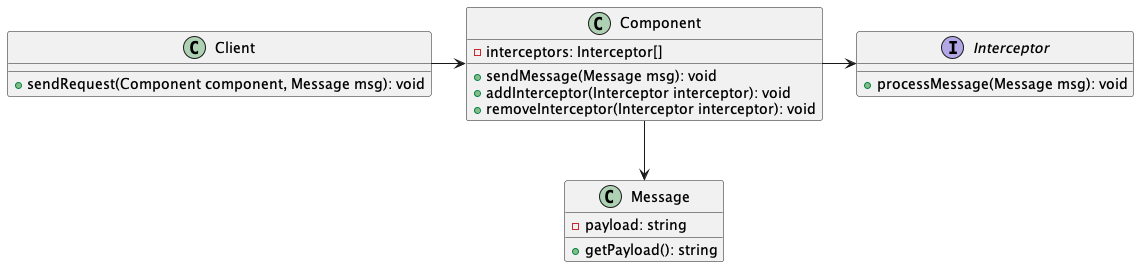
\includegraphics[width=0.99\textwidth]{fig/uml/intercept-class.png}
    \caption{Interceptor Pattern}
    \label{fig:intercept-class}
  \end{figure}
\end{frame}

\begin{frame}
  \frametitle{Interceptor}
  \framesubtitle{Sequenz}
  \begin{figure}[!ht]
    \centering
    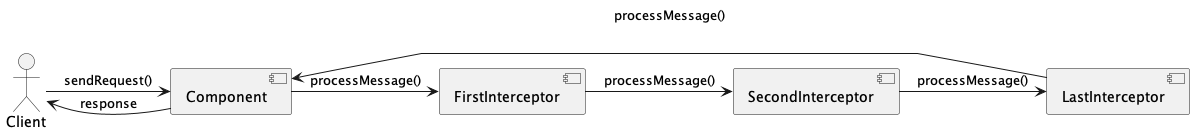
\includegraphics[width=0.99\textwidth]{fig/uml/intercept-seq.png}
    \caption{Interceptor Pattern Sequenz}
    \label{fig:intercept-seq}
  \end{figure}
\end{frame}
%\section{Einleitung}
\subsection{Watchdog}
\begin{frame}
  \frametitle{Watchtog}
  \framesubtitle{Watchdog}
  \begin{itemize}
  \item Überwachung von Ressourcen oder Prozessen in einem System
  \item Erhöht Stabilität und Zuverlässigkeit
  \item Zwei Hauptkomponenten: Watchdog und überwachtes System
  \item Frühzeitige Erkennung und Behebung von Problemen
  \item Anwendbar in verschiedenen Bereichen (z.B. eingebettete Systeme, verteilte Systeme)
  \item Trennung der Verantwortlichkeiten für optimale Effektivität
\end{itemize}
\end{frame}

%\section{Einleitung}
\subsection{Fassade}
\begin{frame}
  \frametitle{Fassade}
  \framesubtitle{Idee}
  \begin{itemize}
    \item Vereinfachte Schnittstelle für den Zugriff 
    \item Reduktion der Komplexität
  \end{itemize}
\end{frame}


\subsection{Pipeline}
\begin{frame}
  \frametitle{Pipeline}
  \framesubtitle{Idee}
  \begin{itemize}
    \item Für komplexe Verarbeitungsprozesse
    \item Sequentielle Ausführung
    \item Spezialisierten Modul (Fetch, Decode, Execute Pipeline)
  \end{itemize}
\end{frame}

\subsection{Master-Worker}
\begin{frame}
  \frametitle{Master-Worker}
  \framesubtitle{Idee}
  \begin{itemize}
    \item Speziell für verteilte Systeme entwickelt
    \item Zentrale Einheit (Master) welcher die Kontrolle über mehrere untergeordnete Einheiten (Worker) hat
    \item Arbeitslast effizient auf mehrere Prozessoren oder Knoten zu verteilen
  \end{itemize}
\end{frame}

% ------------------------------------------------------------------------------
% Fin
\end{document}